\section{Ứng dụng trong Giải tích 1}

\subsection{Phép tính vi phân hàm một biến số}

\subsubsection{Tìm tập xác định của hàm số}

Xét hàm số \( y = \sqrt{2\ln{x} - 3} \). Điều kiện xác định là biểu thức trong hàm $\ln$ phải dương và biểu thức trong căn phải không âm:
\[
\left\{
\begin{aligned}
	&x > 0 \\
	&2\ln{x} - 3 \geq 0 \Rightarrow \ln{x} \geq \frac{3}{2} \Rightarrow x \geq e^{\frac{3}{2}}
\end{aligned}
\right.
\]

Giải điều kiện trong SageMath:
\begin{lstlisting}
	sage: var('x')
	sage: solve(log(x) >= 3/2, x)
	[x >= e^(3/2)]
\end{lstlisting}

Vậy tập xác định của hàm là $D=\left[e^{\frac{3}{2}};+\infty \right)$.

\textbf{Lưu ý:} Hàm \texttt{solve()} trong SageMath có thể trả về kết quả dưới dạng các biểu thức logic hoặc bất phương trình, và bạn có thể áp dụng các hàm như \texttt{find\_root()} hoặc \texttt{plot()} để kiểm tra trực quan kết quả. 

\subsubsection{Tìm miền giá trị của hàm số}

Xét hàm số \( y = \sqrt{1 - \left( \frac{x - 1}{x + 1} \right)^2} \). Tìm miền giá trị của hàm số trên tập (0;2).

\begin{lstlisting}
	sage: var('x')
	sage: f(x) = sqrt(1 - ((x - 1)/(x + 1))^2)
	sage: f.find_local_maximum(0, 2)
	(1.00000000000000, 0.999999967094019)
	sage: f.find_local_minimum(0, 2)
	(0.0001869787205816002, 8.740260678362169e-09)
\end{lstlisting}

Kết quả cho biết trên tập (0;2), tập giá trị của $f(x)$ là \\$(8.740260678362169e-09, 0.999999967094019)
$.

\subsubsection{Làm việc với hàm hyperbolic}
Ví dụ hàm \( f(x) = \sinh(x) + \cosh(x) \):
\begin{lstlisting}
	sage: f(x) = sinh(x) + cosh(x)
	sage: f(1)
	cosh(1) + sinh(1)
	sage: float(f(1))
	2.718281828459045
\end{lstlisting}

\subsubsection{Tìm hàm \( f(x) \)}
Tìm hàm $f(x)$, biết \( f(x + \frac{1}{x}) = x^2 + \frac{1}{x^2} \).\\

Gợi ý biến đổi biểu thức: Đặt \( t = x + \frac{1}{x} \Rightarrow f(t) = t^2 - 2 \).
\begin{lstlisting}
	sage: var('x t')
	sage: t = x + 1/x
	sage: expr = x^2 + 1/x^2
	sage: f_t = simplify((t)^2 - 2)
	sage: f_t
	(x + 1/x)^2 - 2
\end{lstlisting}

\subsubsection{Tìm hàm ngược}

Cho hàm \( y = \frac{1}{2}(e^x - e^{-x}) = \sinh(x) \). Hàm ngược của hàm số này là \( x = \operatorname{arcsinh}(y) \), hay còn gọi là hàm sinh ngược.

Giải phương trình để tìm hàm ngược trong SageMath:

\begin{lstlisting}
	sage: var('x y')
	sage: solve(y == (1/2)*(exp(x) - exp(-x)), x)
	[x == log(y - sqrt(y^2 + 1)), x == log(y + sqrt(y^2 + 1))]
\end{lstlisting}

Kết quả SageMath trả về là:

\[
x = \ln\left( y + \sqrt{y^2 + 1} \right)
\]

Do đó, hàm ngược là:

\[
\boxed{f^{-1}(y) = \ln\left( y + \sqrt{y^2 + 1} \right)}
\]

\subsubsection{Tính giới hạn, kiểm tra tính liên tục}
Xét hàm \( f(x) = \frac{x}{4 - x^2} \) trên khoảng \( [-1,1] \).

Giới hạn tại biên:
\begin{lstlisting}
	sage: limit(x/(4 - x^2), x=1)
	1/3
	sage: limit(x/(4 - x^2), x=-1)
	-1/3
\end{lstlisting}

\subsubsection{Tính đạo hàm, cực trị, tiệm cận}
Cho hàm \( y = x - \ln(1 + x) \):
\begin{lstlisting}
	   sage: f(x) = x - log(1 + x)
	sage: diff(f, x)              # Dao ham cap 1
	x |--> -1/(x + 1) + 1
	sage: diff(f, x, 2)           # Dao ham cap 2
	x |--> (x + 1)^(-2)
	sage: solve(diff(f, x) == 0, x)  # Tim cuc tri
	[x == 0]
	sage: limit(f, x=-oo)	# Tiem can ngang (Gioi han trai)
	x |--> -Infinity
	sage: limit(f, x=+oo)	# Tiem can ngang (Gioi han phai)
	x |--> +Infinity
	sage: limit(f, x=-1)          # Tiem can dung
	x |--> Infinity
\end{lstlisting}

\subsection{Phép tính tích phân hàm một biến số}

\subsubsection{Tính tích phân bất định}
\begin{lstlisting}
	sage: integrate(tan(x)^3, x)
	-1/2/(sin(x)^2 - 1) + 1/2*log(sin(x)^2 - 1)
\end{lstlisting}

\subsubsection{Tính tích phân xác định}
\begin{lstlisting}
	sage: integrate(exp(-x^2), (x, -1, 1))
	sqrt(pi)*erf(1)
\end{lstlisting}

\subsubsection{Tính tích phân suy rộng}
\begin{lstlisting}
	sage: integrate(1/x^2, (x, 1, oo))
	1
\end{lstlisting}

\subsubsection{Tính diện tích hình phẳng}
Diện tích giữa đồ thị \( y = \sin{x} \) và trục hoành từ \( 0 \) đến \( \pi \):
\begin{lstlisting}
	sage: integrate(abs(sin(x)), (x, 0, pi))
	2
\end{lstlisting}

\subsubsection{Thể tích vật thể quay quanh trục hoành}
Cho \( y = \sqrt{x} \), thể tích khi quay quanh trục $Ox$ từ 0 đến 1:
\begin{lstlisting}
	sage: integrate(pi * (sqrt(x))^2, (x, 0, 1))
	1/2*pi
\end{lstlisting}

\subsection{Hàm số nhiều biến số}

\subsubsection{Tính giới hạn hàm nhiều biến}
SageMath không tự động tính giới hạn nhiều biến tại điểm như Mathematica hay Maple.

\subsubsection{Đạo hàm riêng và vi phân toàn phần}
Xét hàm \( f(x, y) = \frac{x^2 y}{x^2 + y^2} \):
\begin{lstlisting}
	sage: var('x y')
	sage: f(x, y) = (x^2 * y)/(x^2 + y^2)
	sage: diff(f, x)	# Dao ham theo bien x
	(x, y) |--> -2*x^3*y/(x^2 + y^2)^2 + 2*x*y/(x^2 + y^2)
	sage: diff(f, y)	# Dao ham theo bien y
	(x, y) |--> -2*x^2*y^2/(x^2 + y^2)^2 + x^2/(x^2 + y^2)
\end{lstlisting}

Kết quả là:
$$f'_x(x,y)=\dfrac{-2x^3y}{x^2 + y^2}+\dfrac{2xy}{x^2 + y^2}$$
$$f'_y(x,y)=\dfrac{-2x^2y^2}{x^2 + y^2}+\dfrac{x^2}{x^2 + y^2}$$

\subsubsection{Khai triển chuỗi Taylor-Maclaurin hàm nhiều biến}
Xét hàm \( f(x, y) =  e^{x+y}\):
\begin{lstlisting}
	sage: var('x y')
	sage: f(x, y) = exp(x + y)
	sage: taylor(f, (x, 0), 3)
	(x, y) |--> 1/6*x^3*e^y + 1/2*x^2*e^y + x*e^y + e^y
\end{lstlisting}

Kết quả là: $\frac{1}{6}x^3e^y + \frac{1}{2}x^2e^y + xe^y + e^y$.

\subsubsection{Vẽ đồ thị hàm số nhiều biến}
\begin{lstlisting}
	sage: var('x y')
	sage: plot3d(sin(x^2 + y^2), (x, -2, 2), (y, -2, 2))
\end{lstlisting}
\begin{figure}[H]
	\centering
	\includegraphics[width=0.7\linewidth]{images/5134}
	\caption{Đồ thị hàm $f(x,y)=sin(x^2+y^2)$ trên $\left[-2,2\right]*\left[-2,2\right]$}
	\label{fig:5134}
\end{figure}

\section{Ứng dụng trong Giải tích 2}

\subsection{Tích phân bội}
\subsubsection{Tính tích phân kép}
Xét tích phân kép:
\[ I = \iint\limits_D (x + y) \, dx \, dy \quad \text{với } D: 0 \le x \le 1, \ 0 \le y \le x \]
Trong SageMath:
\begin{lstlisting}
	sage: var('x y')
	sage: integrate(integrate(x + y, y, 0, x), x, 0, 1)
	1/2		#Ket qua
	sage: # Ve mien D
	sage: region = region_plot(lambda x, y: y <= x and y >= 0 and x >= 0 and x <= 1, (x, 0, 1), (y, 0, 1), incol='lightblue')
	sage: show(region)
\end{lstlisting}
\begin{figure}[H]
	\centering
	\includegraphics[width=0.7\linewidth]{images/5211}
	\caption{Miền $D: 0 \le x \le 1, \ 0 \le y \le x$}
	\label{fig:5211}
\end{figure}

\subsubsection{Toạ độ cực và tích phân trong toạ độ cực}
Xét tích phân:
\[ I = \iint\limits_D (x^2 + y^2) \, dx \, dy \quad \text{với } D \text{ là hình tròn tâm O bán kính 1}
\Rightarrow x = r\cos\theta, \ y = r\sin\theta \]
\begin{lstlisting}
	sage: var('r theta')
	sage: assume(r >= 0)
	sage: integrand = (r^2) * r  # x^2 + y^2 = r^2 va Jacobian la r
	sage: integrate(integrate(integrand, r, 0, 1), theta, 0, 2*pi)
	1/2*pi		# Ket qua
	sage: # Ve mien D
	sage: circle = implicit_plot(x^2 + y^2 == 1, (x, -1.2, 1.2), (y, -1.2, 1.2), color='red')
	sage: region = region_plot(lambda x, y: x^2 + y^2 <= 1, (x, -1, 1), (y, -1, 1), incol='lightgreen')
	show(region + circle)
\end{lstlisting}
\begin{figure}[H]
	\centering
	\includegraphics[width=0.7\linewidth]{images/5212}
	\caption{Miền D được vẽ bằng phương pháp tọa độ cực}
	\label{fig:5212}
\end{figure}

\subsubsection{Tích phân bội ba}
\[ I = \iiint\limits_E z \, dV \quad \text{với } E = \{(x, y, z) \mid 0 \le x \le 1, 0 \le y \le 1 - x, 0 \le z \le x + y \} \]
\begin{lstlisting}
	sage: var('x y z')
	sage: integrate(integrate(integrate(z, z, 0, x + y), y, 0, 1 - x), x, 0, 1)
	1/8		# Ket qua
\end{lstlisting}
\begin{figure}[H]
	\centering
	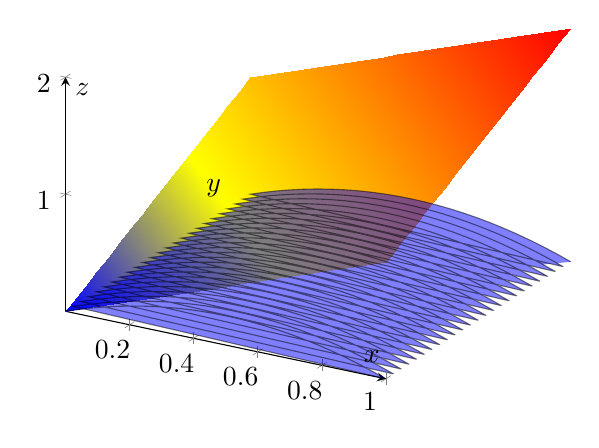
\begin{tikzpicture}
		\begin{axis}[axis lines=middle, xlabel={$x$}, ylabel={$y$}, zlabel={$z$},
			xmin=0, xmax=1, ymin=0, ymax=1, zmin=0, zmax=2,
			domain=0:1, view={30}{30}, width=8cm]
			
			\addplot3[surf, shader=interp] 
			{x + y};
			\addplot3[opacity=0.5, fill=blue] 
			{x*(1-x)};
		\end{axis}
	\end{tikzpicture}
	\caption{Mô phỏng miền tính tích phân bội ba}
	\label{fig:truc-toa-do}
\end{figure}

\subsection{Ứng dụng tích phân bội: diện tích, thể tích}
\subsubsection{Tính diện tích mặt phẳng}
\[ A = \iint\limits_D 1 \, dx \, dy \quad \text{với } D: 0 \le x \le 1, \ 0 \le y \le \sqrt{1 - x^2} \]
\begin{lstlisting}
	sage: integrate(integrate(1, y, 0, sqrt(1 - x^2)), x, 0, 1)
	1/4*pi		# Ket qua
	sage: # Ve mien D
	sage: f(x) = sqrt(1 - x^2)
	sage: p1 = plot(f(x), (x, 0, 1), fill=True, color='lightblue', legend_label="Vung D")
	sage: p1.show()
\end{lstlisting}
\begin{figure}[H]
	\centering
	\includegraphics[width=0.7\linewidth]{images/5221}
	\caption{Miền cần tính diện tích $D: 0 \le x \le 1, \ 0 \le y \le \sqrt{1 - x^2}$}
	\label{fig:5221}
\end{figure}

\subsubsection{Thể tích vật thể}
Thể tích vật thể giới hạn bởi mặt phẳng \( z = x^2 + y^2 \) phía dưới và mặt phẳng \( z = 4 \) phía trên:
\begin{lstlisting}
	sage: var('r theta')
	sage: assume(r >= 0)
	sage: integrand = (4 - r^2) * r  # The tich = \int (z tren - z duoi)*Jacobian
	sage: integrate(integrate(integrand, r, 0, 2), theta, 0, 2*pi)
	8*pi 		# Ket qua 
\end{lstlisting}
\begin{figure}[ht!]
	\centering
	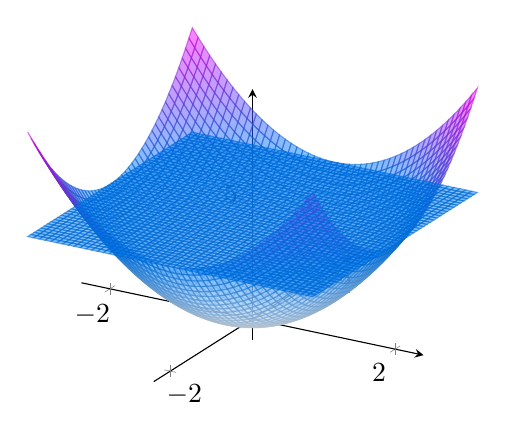
\begin{tikzpicture}
		\begin{axis}[
			axis lines = middle,
			view={30}{30},
			colormap/cool,
			enlargelimits,
			grid=both,
			]
			% Vẽ mặt phẳng z = x^2 + y^2 (phía dưới)
			\addplot3[
			domain=-2:2,
			y domain=-2:2,
			samples=50,
			samples y=50,
			z buffer=sort,
			surf,
			opacity=0.5,
			]
			{x^2 + y^2};
			
			% Vẽ mặt phẳng z = 4 (phía trên)
			\addplot3[
			domain=-2:2,
			y domain=-2:2,
			samples=50,
			samples y=50,
			z buffer=sort,
			surf,
			opacity=0.5,
			]
			{4};
		\end{axis}
	\end{tikzpicture}
	\caption{Mô phỏng miền vật thể giới hạn bởi mặt phẳng \( z = x^2 + y^2 \) phía dưới và mặt phẳng \( z = 4 \) phía trên.}
\end{figure}

\subsubsection{Tích phân phụ thuộc tham số}
\[ I(a) = \int_0^1 \frac{x^a - 1}{\ln x} \, dx \quad (a > 0) \]
\begin{lstlisting}
	sage: var('a x')
	sage: assume(a > 0)
	sage: integral = integrate((x^a - 1)/log(x), x, 0, 1)
	sage: integral
	I*pi + log(a + 1)
\end{lstlisting}

\subsection{Tích phân đường}
\subsubsection{Tích phân đường loại 1}
Tính \( \int_C f(x,y) ds \), với \( C: y = x^2, 0 \le x \le 1 \)
\begin{lstlisting}
	sage: f(x, y) = x + y
	sage: dx = 1
	sage: dy = diff(x^2, x)
	sage: ds = sqrt(dx^2 + dy^2)
	sage: I = integrate(f(x, x^2)*ds, x, 0, 1)
	sage: I
	67/96*sqrt(5) - 1/64*arcsinh(2) - 1/12		#Ket qua
	sage: # Ve mien D
	sage: var('x y')
	sage: f(x) = x^2
	sage: plot1 = plot(f(x), (x, 0, 1), color='blue', sage: legend_label='y = x^2')
	sage: f_xy(x, y) = x + y
	sage: plot1.show()
	
\end{lstlisting}
\begin{figure}[H]
	\centering
	\includegraphics[width=0.5\linewidth]{images/5231}
	\caption{Miền $C: y = x^2, 0 \le x \le 1$}
	\label{fig:5231}
\end{figure}


\subsubsection{Tích phân đường loại 2}
Tính \( \int_C (x \, dx + y \, dy) \), với \( C \) là đường tròn đơn vị.
\begin{lstlisting}
	sage: x(t) = cos(t)
	sage: y(t) = sin(t)
	sage: dx = diff(x(t), t)
	sage: dy = diff(y(t), t)
	sage: integrand = x(t)*dx + y(t)*dy
	sage: integrate(integrand, t, 0, 2*pi)
	0		# Ket qua
	sage: # Ve mien D
	sage: var('t')
	sage: x(t) = cos(t)
	sage: y(t) = sin(t)
	sage: parametric_plot((x(t), y(t)), (t, 0, 2*pi), color='blue', legend_label='C: x(t), y(t)')
\end{lstlisting}
\begin{figure}[H]
	\centering
	\includegraphics[width=0.5\linewidth]{images/5232}
	\caption{Miền $C$ là đường tròn đơn vị}
	\label{fig:5232}
\end{figure}


\subsection{Tích phân mặt}
Tính tích phân mặt của hàm \( f(x, y, z) = z \) trên mặt phẳng \( z = 1 - x - y, 0 \le x, y \le 1, x + y \le 1 \)
\begin{lstlisting}
	sage: z(x, y) = 1 - x - y
	sage: f(x, y) = z(x, y)
	sage: I = integrate(integrate(f(x, y), y, 0, 1 - x), x, 0, 1)
	sage: I
	1/6		# Ket qua
\end{lstlisting}
\begin{figure}[H]
	\centering
	\tdplotsetmaincoords{70}{120}
	\begin{tikzpicture}[tdplot_main_coords, scale=5]
		
		% Trục tọa độ
		\draw[->] (0,0,0) -- (1.1,0,0) node[anchor=north east]{$x$};
		\draw[->] (0,0,0) -- (0,1.1,0) node[anchor=north west]{$y$};
		\draw[->] (0,0,0) -- (0,0,1.1) node[anchor=south]{$z$};
		
		% Các điểm tam giác
		\coordinate (A) at (1,0,0);
		\coordinate (B) at (0,1,0);
		\coordinate (C) at (0,0,1);
		
		% Mặt phẳng z = 1 - x - y là tam giác ABC
		\filldraw[fill=blue!30, opacity=0.7] (A) -- (B) -- (C) -- cycle;
		
		% Nhãn điểm
		\node at (A) [below right] {$(1,0,0)$};
		\node at (B) [above left] {$(0,1,0)$};
		\node at (C) [above right] {$(0,0,1)$};
		
	\end{tikzpicture}
	\caption{Mặt phẳng $z = 1 - x - y$ trên miền tam giác $x + y \leq 1$}
\end{figure}

\subsection{Lý thuyết trường}
\subsubsection{Đạo hàm theo hướng}
Tính đạo hàm theo hướng của \( f(x, y) = x^2y \) tại \( A(1, 2) \) theo hướng \( \vec{v} = (3, 4) \)
\begin{lstlisting}
	sage: f(x, y) = x^2*y
	sage: u = vector([3, 4]).normalized()
	sage: grad_f = vector([diff(f(x, y), x), diff(f(x, y), y)])
	sage: point = vector([1, 2])
	sage: grad_at_A = grad_f.subs(x=point[0], y=point[1])
	sage: directional_derivative = grad_at_A.dot_product(u)
	sage: directional_derivative
	16/5	# Ket qua
	
	sage: # Ve mien D
	sage: var('x y')
	sage: # Ham so
	sage: f(x, y) = x^2 * y
	sage: # Diem A
	sage: A = vector([1, 2])
	sage: # Vector huong
	sage: v = vector([3, 4])
	sage: u = v.normalized()
	sage: # Gradient
	sage: grad_f = vector([diff(f(x, y), x), diff(f(x, y), y)])
	sage: grad_A = grad_f.subs(x=A[0], y=A[1])
	sage: # Vector dao ham theo huong
	sage: D_u_f = grad_A.dot_product(u)
	sage: vec_D = D_u_f * u
	sage: # Ve mat ham
	sage: surface = plot3d(f(x, y), (x, 0, 2), (y, 0, sage: 2), opacity=0.6, color='lightblue')
	sage: # Ve diem A tren mat
	sage: pointA = point3d((A[0], A[1], f(*A)), color='red', size=30)
	sage: # Ve gradient tai A
	sage: grad_arrow = arrow3d((A[0], A[1], f(*A)), (A[0] + grad_A[0], A[1] + grad_A[1], f(*A)), color='green', width=2)
	sage: # Ve vector huong tai A
	sage: u_arrow = arrow3d((A[0], A[1], f(*A)), (A[0] + u[0], A[1] + u[1], f(*A)), color='orange', width=2)
	sage: # Ve vector dao ham theo huong (chi phan vector tren mat, khong tang do cao)
	sage: vecD_arrow = arrow3d((A[0], A[1], f(*A)), (A[0] + vec_D[0], A[1] + vec_D[1], f(*A)), color='purple', width=2)
	sage: # Gop cac thanh phan
	sage: show(surface + pointA + grad_arrow + u_arrow + vecD_arrow, frame=True)
	
\end{lstlisting}
\begin{figure}[H]
	\centering
	\includegraphics[width=0.7\linewidth]{images/5251}
	\caption{Đồ thị mô phỏng đạo hàm theo hướng của \( f(x, y) = x^2y \) tại \( A(1, 2) \) theo hướng \( \vec{v} = (3, 4) \)}
	\label{fig:5251}
\end{figure}

\subsubsection{Tính gradient}
\begin{lstlisting}
	sage: var('x y')
	sage: f(x, y) = x^2 * y
	sage: # Tinh gradient thu cong
	sage: grad_f = vector([diff(f(x, y), x), diff(f(x, y), y)])
	sage: grad_f
	(2*x*y, x^2)
\end{lstlisting}

\newpage
\section{Ứng dụng trong Giải tích 3}

\subsection{Chuỗi số, xét sự hội tụ của chuỗi số}
Xét sự hội tụ của chuỗi: $\sum_{n=1}^{\infty} \dfrac{1}{n^p}$ với $p>1$.
\begin{lstlisting}
	sage: var('n')
	sage: f = 1/n^100
	sage: sum(f, n, 1, oo)
	sage: var('n')
	sage: f = 1/n^100
	sage: sum(f, n, 1, oo)
	189196075638244.../981520542075751...*pi^100	# Ket qua +oo
\end{lstlisting}

\subsection{Chuỗi hàm, tính tổng chuỗi, chuỗi hội tụ đều}
Tính tổng chuỗi hàm $\sum_{n=0}^{\infty}{\dfrac{x^n}{n!}}$
\begin{lstlisting}
	sage: var('x n')
	sage: f = x^n/factorial(n)
	sage: S = sum(f, n, 0, oo)
	sage: S
	e^x			# Ket qua
\end{lstlisting}

\subsection{Chuỗi lũy thừa, khai triển Taylor, Maclaurin}
Khai triển chuỗi Maclaurin của $\sin{x}$.
\begin{lstlisting}
	sage: taylor(sin(x), x, 0, 7)
	-1/5040*x^7 + 1/120*x^5 - 1/6*x^3 + x		# Ket qua
\end{lstlisting}

\subsection{Chuỗi Fourier, khai triển Fourier}
Khai triển chuỗi Fourier của $f(x)=x$ trên $\left[-\pi,\pi\right]$.
\begin{lstlisting}
	sage: var('x n')
	sage: f(x) = x
	sage: a0 = (1/pi)*integrate(f(x), x, -pi, pi)
	sage: a0
	0
	sage: an = (1/pi)*integrate(f(x)*cos(n*x), x, -pi, pi)
	sage: an
	0
	sage: bn = (1/pi)*integrate(f(x)*sin(n*x), x, -pi, pi)
	sage: bn
	-2*(pi*n*cos(pi*n) - sin(pi*n))/(pi*n^2)

	# Ve do thi khai trien Fourier bac 5
	sage: fourier = sum(2*(-1)^(k+1)/k*sin(k*x) for k in (1..5))
	sage: p1 = plot(f(x), (x, -pi, pi), color='blue', legend_label='f(x)=x')
	sage: p2 = plot(fourier, (x, -pi, pi), color='red', legend_label='Fourier')
	sage: show(p1 + p2)
\end{lstlisting}
\begin{figure}[H]
	\centering
	\includegraphics[width=0.7\linewidth]{images/534}
	\caption{Đồ thị minh họa khai triển chuỗi Fourier của $f(x)=x$ trên $\left[-\pi,\pi\right]$}
	\label{fig:534}
\end{figure}


\subsection{Giải phương trình vi phân tuyến tính cấp 1, cấp 2}
Giải phương trình:
\[
y' + y = e^x
\]
\begin{lstlisting}
	sage: var('x y')
	sage: y = function('y')(x)
	sage: de = diff(y, x) + y == e^x
	sage: desolve(de, y)
	1/2*(2*_C + e^(2*x))*e^(-x)		# Ket qua
\end{lstlisting}
Giải phương trình:
\[
y'' - y = 0
\]	
\begin{lstlisting}
	sage: y = function('y')(x)
	sage: de2 = diff(y, x, 2) - y == 0
	sage: desolve(de2, y)
	_K2*e^(-x) + _K1*e^x		# Ket qua
\end{lstlisting}

\subsection{Giải phương trình Euler}
Giải phương trình vi phân Euler:
\[
x^2 y'' - x y' + y = 0
\]
\begin{lstlisting}
	sage: y = function('y')(x)
	sage: de = x^2*diff(y, x, 2) - x*diff(y, x) + y == 0
	sage: desolve(de, y)
	(_K2*log(x) + _K1)*x		# Ket qua
\end{lstlisting}

\subsection{Giải hệ phương trình vi phân cấp 1}
Giải hệ:
\[
\begin{cases}
	x' = x + y \\
	y' = x - y
\end{cases}
\]
\begin{lstlisting}
	sage: t = var('t')
	sage: x = function('x')(t)
	sage: y = function('y')(t)
	sage: de1 = diff(x, t) == x + y
	sage: de2 = diff(y, t) == x - y
	sage: desolve_system([de1, de2], [x, y])
	[x(t) == 1/2*sqrt(2)*(x(0) + y(0))*sinh(sqrt(2)*t) + cosh(sqrt(2)*t)*x(0),
	y(t) == 1/2*sqrt(2)*(x(0) - y(0))*sinh(sqrt(2)*t) + cosh(sqrt(2)*t)*y(0)]
\end{lstlisting}

\subsection{Biến đổi Laplace, ứng dụng giải phương trình vi phân}
Giải phương trình bằng biến đổi Laplace:
\[
y'' + y = \sin(t), \quad y(0) = 0,\ y'(0) = 1
\] 
\begin{lstlisting}
	sage: var('t s')
	sage: y = function('y')(t)
	sage: de = diff(y, t, 2) + y == sin(t)
	sage: desolve_laplace(de, y, ivar=t)
	-1/2*t*cos(t) + 1/2*(2*D[0](y)(0) + 1)*sin(t) + cos(t)*y(0)		# Ket qua
\end{lstlisting}

\section{Ứng dụng trong Đại số tuyến tính}

\subsection{Các phép toán Logic, tập hợp}
Các phép toán logic và phép toán trên tập hợp có thể được thực hiện bằng các công cụ trong SageMath. Ví dụ, để tính toán hợp, giao, hiệu của các tập hợp, hoặc thực hiện các phép toán logic như AND, OR, NOT, ta có thể sử dụng cú pháp sau.

\begin{lstlisting}
	sage: # Hop va giao cua tap hop
	sage: A = Set([1, 2, 3])
	sage: B = Set([3, 4, 5])
	sage: A.union(B)  # Hop
	{1, 2, 3, 4, 5}
	sage: A.intersection(B)  # Giao
	{3}
\end{lstlisting}

\subsection{Ánh xạ, tìm ảnh và nghịch ảnh}
Để tính ảnh và nghịch ảnh trong ánh xạ, ta có thể áp dụng trực tiếp công thức của ánh xạ. Ví dụ dưới đây minh họa cách tìm ảnh và nghịch ảnh của một số trong ánh xạ \( f(x) = x^2 \).

\begin{lstlisting}
	sage: var('x')
	sage: f = x^2
	sage: f(x=3)  # Tinh anh cua 3
	9
	sage: f.inverse_function()(9)  # Tim nghich anh cua 9
\end{lstlisting}

\subsection{Cấu trúc đại số nhóm, vành, trường, nhóm Abel}
Các phép toán trong các cấu trúc đại số như nhóm, vành và trường có thể thực hiện thông qua các phép toán trong SageMath. Các phép toán nhóm Abel có thể sử dụng phép toán nhóm trong Sage.

\begin{lstlisting}
	# Phep toan nhom Abel
	G = Group([(1, 1), (2, 2)])
	G * G  # Nhan nhom
\end{lstlisting}

\subsection{Số phức, tính module, phép toán số phức, thu gọn về dạng chính tắc}
Các phép toán với số phức như cộng, trừ, nhân, chia, tính module và thu gọn về dạng chính tắc có thể thực hiện trong SageMath. Dưới đây là cách tính module và thu gọn số phức về dạng chính tắc.

\begin{lstlisting}
	sage: z = 3 + 4*I  # So phuc
	sage: abs(z)  # Tinh module
	5
	sage: conjugate(z)  # Tinh phan ao
	11/3
\end{lstlisting}

\subsection{Tìm căn bậc n của số phức, giải phương trình nghiệm phức}
Để tìm căn bậc n của số phức hoặc giải phương trình nghiệm phức, ta sử dụng các hàm \texttt{nth\_root} và \texttt{solve}.

\begin{lstlisting}
	sage: z = 1 + I
	sage: nth_root(z, 3)  # Tim can bac 3 cua z
	sage: solve(x^2 + 1 == 0, x)  # Giai phuong trinh x^2 + 1 = 0
\end{lstlisting}

\subsection{Ma trận và các phép toán ma trận, định thức, ma trận nghịch đảo, ma trận mũ, hạng của ma trận, hệ phương trình tuyến tính (Phương pháp Gauss)}
Các phép toán ma trận như tính định thức, nghịch đảo, ma trận mũ và hạng có thể thực hiện dễ dàng trong SageMath. Hệ phương trình tuyến tính có thể giải bằng phương pháp Gauss.

\begin{lstlisting}
	sage: A = Matrix([[1, 2], [3, 4]])
	sage: det(A)  # Tinh dinh thuc
	sage: A.inv()  # Tinh ma tran nghich dao
	sage: A^2  # Ma tran mu
	sage: A.rank()  # Hang cua ma tran
	sage: solve(A*x == [1, 2], x)  # Giai he phuong trinh tuyen tinh
\end{lstlisting}

\subsection{Không gian vector, kiểm tra hệ độc lập tuyến tính}
Để kiểm tra tính độc lập tuyến tính của các vector, ta có thể tính hạng của ma trận tạo thành từ các vector đó.

\begin{lstlisting}
	sage: v1 = vector([1, 2])
	sage: v2 = vector([2, 4])
	sage: matrix([v1, v2]).rank()  # Kiem tra tinh doc lap tuyen tinh
\end{lstlisting}

\subsection{Tìm cơ sở và số chiều sinh bởi hệ vector}
Cơ sở của không gian vector có thể tìm được thông qua phép biến đổi ma trận, ví dụ dưới đây minh họa cách tìm cơ sở và số chiều sinh bởi hệ vector.

\begin{lstlisting}
	sage: v1 = vector([1, 0])
	sage: v2 = vector([0, 1])
	sage: matrix([v1, v2]).column_space()  # Tim co so
\end{lstlisting}

\subsection{Ánh xạ tuyến tính, giá trị riêng và vector riêng}
Các phép toán như tìm giá trị riêng và vector riêng của một ma trận có thể được thực hiện qua hàm `eigenvalues` và `eigenvectors`.

\begin{lstlisting}
	sage: A = Matrix([[1, 2], [3, 4]])
	sage: A.eigenvalues()  # Tinh gia tri rieng
	sage: A.eigenvectors()  # Tinh vector rieng
\end{lstlisting}

\subsection{Chéo hóa ma trận}
Chéo hóa ma trận có thể thực hiện bằng cách sử dụng hàm `diagonalize`, nếu ma trận có đủ số lượng vector riêng độc lập.

\begin{lstlisting}
	sage: A = Matrix([[4, 1], [2, 3]])
	sage: A.diagonalize()  # Cheo hoa ma tran
\end{lstlisting}

\subsection{Trực chuẩn hóa cơ sở, xác định ma trận chuyển cơ sở, tìm hình chiếu trực giao}
Các phép toán như chuẩn hóa cơ sở, ma trận chuyển cơ sở và hình chiếu trực giao có thể thực hiện bằng các phép toán ma trận và vector trong SageMath.

\begin{lstlisting}
	sage: v1 = vector([1, 0])
	sage: v2 = vector([0, 1])
	sage: v1.normalized()  # Chuan hoa vector
	sage: projection = v1.project_onto(v2)  # Tinh hinh chieu truc giao
\end{lstlisting}

\subsection{Vẽ các đường cong phẳng, mặt bậc hai}
Để vẽ các đường cong phẳng và mặt bậc hai, ta có thể sử dụng các hàm vẽ 2D và 3D trong SageMath. Dưới đây là cách vẽ đường cong và mặt bậc hai.

\begin{lstlisting}
	sage: plot(x^2 + y^2, (x, -2, 2), (y, -2, 2))  # Ve duong cong
	sage: implicit_plot3d(x^2 + y^2 - z, (x, -2, 2), (y, -2, 2), (z, 0, 10))  # Ve mat bac hai
\end{lstlisting}

\section{Ứng dụng trong Xác suất thống kê}

\subsection{Tổ hợp, chỉnh hợp, giai thừa}
SageMath hỗ trợ các hàm tính tổ hợp và giai thừa để giải các bài toán xác suất. Tuy nhiên, SageMath không có sẵn hàm tính chỉnh hợp, nên ta sẽ sử dụng cách tính theo đúng công thức $P(n,k)=\dfrac{n!}{(n-k)!}$.

\begin{lstlisting}
	# Tinh giai thua
	sage: factorial(5)
	120
	
	# Tinh to hop chap 3 cua 5
	sage: binomial(5, 3)
	10
	
	# Tinh chinh hop chap 2 cua 4
	sage: factorial(4) / factorial(4 - 2)
	12
\end{lstlisting}

\subsection{Biến ngẫu nhiên và phân phối xác suất}
SageMath có các hàm tích hợp để tính kỳ vọng, phương sai và độ lệch chuẩn của các biến ngẫu nhiên.

\begin{lstlisting}
	# Tinh ky vong va phuong sai cua bien ngau nhien
	sage: var('x p')
	sage: X = [1, 2, 3]
	sage: P = [0.2, 0.5, 0.3]
	sage: mean = sum(x * p for x, p in zip(X, P))
	sage: variance = sum((x - mean)^2 * p for x, p in zip(X, P))
	sage: mean, variance
	(2.10000000000000, 0.490000000000000)
\end{lstlisting}

Ta cũng có thể sử dụng từ thư viện \texttt{NumPy} để tính giá trị trung bình (mean), phương sai (variance) và độ lệch chuẩn như sau:
\begin{lstlisting}
	# Tinh ky vong va phuong sai cua bien ngau nhien voi NumPy
	sage: import numpy as np
	sage: data = [10, 20, 30, 40, 50]
	sage: mean = np.mean(data)
	sage: variance = np.var(data)
	sage: std_dev = np.std(data)
	sage: mean, variance, std_dev
	(30.0, 200.0, 14.142135623730951)
\end{lstlisting}
Hoặc sử dụng hàm từ \texttt{SciPy}:
\begin{lstlisting}
	# Tinh ky vong va phuong sai cua bien ngau nhien voi SciPy
	sage: from scipy.stats import describe
	sage: data = [10, 20, 30, 40, 50]
	sage: stats = describe(data)
	sage: stats.mean, stats.variance
	(30.0, 200.0)
\end{lstlisting}

\subsubsection{Vẽ đồ thị phân phối xác suất}
Dưới đây là ví dụ vẽ đồ thị phân phối nhị thức với SageMath.

\begin{lstlisting}
	# Ve do thi phan phoi nhi thuc voi p = 0.5, n = 10
	sage: var('k')
	sage: p = 0.5
	sage: n = 10
	sage: P = [binomial(n, k) * p^k * (1 - p)^(n - k) for k in range(n + 1)]
	sage: bar_chart(P, width=0.5, title='Phan phoi nhi thuc', axes=True)
\end{lstlisting}
\begin{figure}[H]
	\centering
	\includegraphics[width=0.7\linewidth]{images/screenshot001}
	\caption{Biểu đồ phân phối nhị thức với $(n,p)=(10,0.5)$}
	\label{fig:screenshot001}
\end{figure}

\subsection{Biến ngẫu nhiên nhiều chiều}
Tính hàm mật độ xác suất biên và xác suất điều kiện.

\begin{lstlisting}
	# Phan phoi xac suat bien
	sage: var('x y')
	sage: f = x * y
	sage: integrate(f, (x, 0, 1))  # Ham mat do xac suat bien theo y
	1/2 * y^2
\end{lstlisting}

\subsection{Ước lượng tham số}
Tính khoảng tin cậy cho kỳ vọng và tỷ lệ.

\begin{lstlisting}
	# Uoc luong ky vong voi do tin cay 95%
	sage: var('x n s')
	sage: mu = x + 1.96 * s / sqrt(n)
	sage: mu.subs({x: 50, s: 10, n: 100})
	51.9600000000000
\end{lstlisting}

\subsection{Kiểm định giả thuyết}
Thực hiện kiểm định giả thuyết với mẫu và tính p-value.

\begin{lstlisting}
	# Kiem dinh Z
	sage: var('xbar mu sigma n')
	sage: Z = (xbar - mu) / (sigma / sqrt(n))
	sage: Z.subs({xbar: 110, mu: 100, sigma: 15, n: 30})
	3.651483716701107
\end{lstlisting}

\subsection{Thống kê mô tả và suy diễn}
Tính các tham số thống kê như trung bình, phương sai, độ lệch chuẩn.

\begin{lstlisting}
	# Thong ke mo ta voi scipy
	sage: from scipy.stats import describe
	sage: data = [10, 20, 30, 40, 50]
	sage: describe(data)
	# Ket qua: N, min, max, mean, variance
	DescribeResult(nobs=5, minmax=(10, 50), mean=30.0, variance=250.0, skewness=0.0, kurtosis=-1.3)
\end{lstlisting}

\subsection{Phân tích hồi quy}
Hồi quy tuyến tính và kiểm định độ phù hợp của mô hình.

\begin{lstlisting}
	# Hoi quy tuyen tinh
	sage: var('x')
	sage: data = [(1, 2), (2, 4), (3, 6)]
	sage: m, b = var('m b')
	sage: model = m * x + b
	sage: eqs = [model.subs(x=xv) == yv for xv, yv in data]
	sage: solve(eqs, m, b)
	[[m == 2, b == 0]]
\end{lstlisting}

\subsection{Phân tích phương sai (ANOVA)}
Phân tích phương sai để kiểm định giả thuyết về nhiều trung bình.

\begin{lstlisting}
	# Phan tich ANOVA
	sage: from scipy.stats import f_oneway
	sage: group1 = [23, 20, 25, 22]
	sage: group2 = [27, 29, 30, 28]
	sage: f_oneway(group1, group2)
	# Ket qua: p-value va thong ke F
	F_onewayResult(statistic=24.0, pvalue=0.002713682035093796)
\end{lstlisting}
